\newpage

\section{Taxicab Distance}
In this activity, we explore \emph{City Geometry}, where points are Euclidean points, given with coordinates; lines are Euclidean lines, defined with equations or by two points, as in Euclidean coordinate geometry; and angles are Euclidean angles.  Distance, however, is measured according to the path a taxicab might travel.  Let's get started.  
\begin{prob}
Suppose we are in a city that is neatly laid out in blocks of two-way streets, with streets running north-south and east-west, and suppose we want to travel from point $A$ to point $B$ in the figure below.  
\[
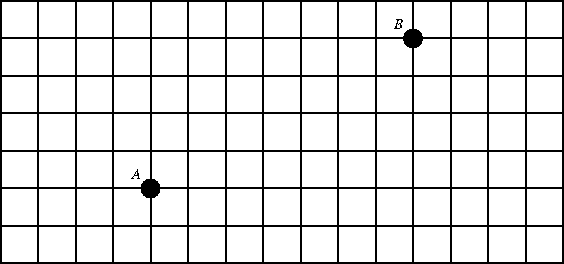
\includegraphics[scale=0.9]{../graphics/citygrideg1.pdf}
\]
\begin{enumerate}
\item What is the \emph{taxicab distance}, measured in city blocks, from point $A$ to point $B$?  (Do we mean the shortest distance, the longest distance, or something else?)  
\item Is there a single shortest path for the taxi to take?  Explain.  
\item Let $A = (1,2)$. What would be the coordinates of $B$?  
\item Describe a calculation that yields the taxicab distance between points $A$ and $B$.  
\item Suppose the taxicab may travel on alleys also running north-south and east-west.  Better yet, suppose the taxicab can create alleys wherever they would be most useful, except that they must still run north-south or east-west.  What then would be the taxicab distance from $A$ to $B$?  Explain.  
\item Based on your reasoning, given points $P = (x_1, y_1)$ and $Q= (x_2, y_2)$, write a formula for, $d_T(P,Q)$, the \emph{taxicab distance} between points $P$ and $Q$.  Check that it works for several pairs of points.  
\end{enumerate}
\end{prob}

\begin{teachingnote}
Continue in section 6.1.1. Also note that section 6.2 includes the paradox of $\sqrt{2}=2$ from the diagonal of a unit square in city geometry.
\end{teachingnote}
  


